% \documentclass[12pt]{article}
% \usepackage[english]{babel}
% \usepackage{natbib}
% \usepackage{url}
% \usepackage[utf8x]{inputenc}
% \usepackage{amsmath}
% \usepackage{graphicx}
% \graphicspath{{images/}}
% \usepackage{parskip}
% \usepackage{fancyhdr}
% \usepackage{vmargin}
% \usepackage{hyperref}
% \usepackage{listings}
% \usepackage{color}
% \usepackage{float}
% \usepackage{fourier}

% \DeclareRobustCommand{\bigO}{%
%   \text{\usefont{OMS}{cmsy}{m}{n}O}%
% }

% \definecolor{dkgreen}{rgb}{0,0.6,0}
% \definecolor{gray}{rgb}{0.5,0.5,0.5}
% \definecolor{mauve}{rgb}{0.58,0,0.82}

% \lstset{frame=tb,
%   language=Python,
%   aboveskip=3mm,
%   belowskip=3mm,
%   showstringspaces=false,
%   columns=flexible,
%   basicstyle={\small\ttfamily},
%   numbers=none,
%   numberstyle=\tiny\color{gray},
%   keywordstyle=\color{blue},
%   commentstyle=\color{dkgreen},
%   stringstyle=\color{mauve},
%   breaklines=true,
%   breakatwhitespace=true,
%   tabsize=3
% }

\documentclass[a4paper, 11pt]{article}

\usepackage{parskip}
\usepackage{hyperref}
\hypersetup{ colorlinks, citecolor=green, filecolor=black, linkcolor=blue, urlcolor=blue } 

\usepackage{colortbl}

\usepackage{amsfonts}

\usepackage[left=2cm, right=2cm, top=2cm]{geometry}
\usepackage{float}
\usepackage{afterpage}
\usepackage{multirow}
\usepackage{listings}
\usepackage{xcolor}
 
\definecolor{codegreen}{rgb}{0,0.6,0}
\definecolor{codegray}{rgb}{0.5,0.5,0.5}
\definecolor{codepurple}{rgb}{0.58,0,0.82}
\definecolor{backcolour}{rgb}{0.95,0.95,0.92}
 
\lstdefinestyle{mystyle}{
    backgroundcolor=\color{backcolour},   
    commentstyle=\color{codegreen},
    keywordstyle=\color{magenta},
    numberstyle=\tiny\color{codegray},
    stringstyle=\color{codepurple},
    basicstyle=\ttfamily\footnotesize,
    breakatwhitespace=false,         
    breaklines=true,                 
    captionpos=b,                    
    keepspaces=true,                 
    numbers=left,                    
    numbersep=5pt,                  
    showspaces=false,                
    showstringspaces=false,
    showtabs=false,                  
    tabsize=2
}
\lstset{style=mystyle}

\usepackage{gensymb}
\usepackage{amsmath}
\usepackage{graphicx}
\usepackage{subfigure}
\usepackage{textcomp}
\usepackage{enumitem}

\newcommand{\points}[1]{(\textbf{#1 marks}) }
\newcommand{\vecthree}[3]{\begin{pmatrix} #1 \\ #2 \\ #3 \end{pmatrix}}
\newcommand{\vecfour}[4]{\begin{pmatrix} #1 \\ #2 \\ #3 \\ #4\end{pmatrix}}
\newcommand{\mat}[1]{\boldsymbol { \mathsf{#1}} }

\DeclareMathOperator*{\argmax}{arg\,max}
\DeclareMathOperator*{\argmin}{arg\,min}
\newcommand{\norm}[1]{\lVert#1\rVert}
\newcommand{\R}{\mathbb{R}}

\definecolor{mycolor}{rgb}{0,0.6,0.5}

% \setmarginsrb{3 cm}{2.5 cm}{3 cm}{2.5 cm}{1 cm}{1.5 cm}{1 cm}{1.5 cm}

\title{Analyzing 0/1 Knapsack Problem Algorithm Design Paradigms}								% Title
\author{M. H. Shaikh, H. F. Ahmed, H. F. Ahmed, K. Abbasi, F. A. Khan}								% Author
\date{\today}											% Date
\makeatletter
\let\thetitle\@title
\let\theauthor\@author
\let\thedate\@date
\makeatother

% \pagestyle{fancy}
% \fancyhf{}
% \chead{\thetitle}
% \cfoot{\thepage}

\begin{document}

%%%%%%%%%%%%%%%%%%%%%%%%%%%%%%%%%%%%%%%%%%%%%%%%%%%%%%%%%%%%%%%%%%%%%%%%%%%%%%%%%%%%%%%%%

\begin{titlepage}
	\centering
    \vspace*{0.5 cm}
    
\includegraphics[scale = 0.47]{logo.png}\\[1.0 cm]	% University Logo
    \textsc{\LARGE Habib University}\\[1.0 cm]	% University Name
	\textsc{\Large CS412}\\[0.5 cm]				% Course Code
	\textsc{\large Design and Analysis of Algorithms}\\[0.5 cm]				% Course Name
	\rule{\linewidth}{0.2 mm} \\[0.4 cm]
	{ \huge \bfseries \thetitle}\\
	\rule{\linewidth}{0.2 mm} \\[0.5 cm]
	{Abbasi, Kainat :
            \texttt{ka04051@st.habib.edu.pk}} \\
    {Feroz, Huda :
    \texttt{ha04081@st.habib.edu.pk}} \\
    {Feroz, Hareem :
    \texttt{hf04097@st.habib.edu.pk}} \\
    {Khan, Faraz :
            \texttt{fk03983@st.habib.edu.pk}} \\
	{Shaikh, Mudasir :
            \texttt{ms03831@st.habib.edu.pk}} \\
	\rule{\linewidth}{0.2 mm} \\[0.5 cm]
	{Submitted to:}\\
			Dr. Shahid  Hussain \\ 
	{\large \thedate}\\[2 cm]
	\vfill
	
\end{titlepage}

\begin{center}
\section*{Abstract}
\end{center}
The aim of this paper is to analyze different approaches taken to solve the Knapsack Problem. The knapsack problem or rucksack problem is a problem in combinatorial optimization: Given a set of items, each with a weight and a value, determine the number of each item to include in a collection so that the total weight is less than or equal to a given limit and the total value is as large as possible. The decision problem form of the knapsack problem is NP-complete, whereas the optimization problem is NP-hard. This paper shall focus on knapsack optimization problem. \\ \\
The paper shall present a comparative analysis of brute force, dynamic programming, memory functions, greedy, genetic, and randomized algorithms. The paper presents complexity analysis of these approaches in view of time and space (memory access). Furthermore, the paper discusses and specifies the limitations of the algorithm approaches. The experimental results show that Dynamic Programming is the best approach if we consider time, space, and optimality. Some algorithms, such as genetic and memory functions save some space, but memory functions take considerably more time than Dynamic Programming whereas genetic doesn't guarantee optimality.

%%%%%%%%%%%%%%%%%%%%%%%%%%%%%%%%%%%%%%%%%%%%%%%%%%%%%%%%%%%%%%%%%%%%%%%%%%%%%%%%%%%%%%%%%

\pagebreak
\tableofcontents
\pagebreak

%%%%%%%%%%%%%%%%%%%%%%%%%%%%%%%%%%%%%%%%%%%%%%%%%%%%%%%%%%%%%%%%%%%%%%%%%%%%%%%%%%%%%%%%%
\section{Introduction}
The goal of the knapsack problem is to maximize the profit without extending the capacity. This project focuses on 0/1 knapsack problem which is a binary problem, i.e. either the decision maker is allowed to pick (1) or not to pick (0) the item, which mean that the items are not dividable. This project shall use brute force algorithm, greedy algorithm, dynamic programming algorithm, genetic algorithm, memory functions, and randomized algorithm (simulated annealing). The aim of this discussion is to find the best algorithm and limitations of these algorithms by comparative analysis.

%%%%%%%%%%%%%%%%%%%%%%%%%%%%%%%%%%%%%%%%%%%%%%%%%%%%%%%%%%%%%%%%%%%%%%%%%%%%%%%%%%%%%%%%%

\section{Resources Utilized}
For the entirety of the project and this report, the following resources were utilized:
\begin{itemize}
    \item Python 3.
    \item matplotlib
    \item \LaTeX
    \item GitHub
    \item numpy
\end{itemize}
%%%%%%%%%%%%%%%%%%%%%%%%%%%%%%%%%%%%%%%%%%%%%%%%%%%%%%%%%%%%%%%%%%%%%%%%%%%%%%%%%%%%%%%%%

\section{Algorithms}



\subsection{Brute Force Algorithm}
The Brute Force algorithm to the knapsack problem generates all possible solutions by generating the power set of the items available. A loop then iterates over the power set and generates the total weight and value for that solution. Each iteration assigns a set as the best solution if it is better than the last best result. In this way, the best solution is returned as the final output. \\
The complexity to generate the power set of all items is $O(2^n)$ and for every solution the complexity for generating the weights and value is $O(n)$. Therefore the algorithmic complexity of this approach is $O(n2^n)$.


\subsection{Greedy Algorithm}
This algorithm solves the problem by choosing the items with as high a value per weight as possible which is a greedy approach. Firstly, we take value-to-weight ratio i.e $v_i$/$w_i$ for i = 1,..,number of items. Then, the algorithm sorts the list of the ratios in decreasing order. For the items in the sorted list, the items, $I_i$ where i=1,...,number of items ,are added to the knapsack if their weight is less than the knapsack's capacity. \\
The complexity to sort the list is $O(n \log n)$ while the complexity to find and then add item $I_i$ in the knapsack is $O(n)$ so the total worst case complexity is $O(n \log n)$.
\subsection{Dynamic Programming Algorithm}
The algorithm solves the problem by breaking it down into simpler sub-problems, and utilizing the fact that the optimal solution to the overall problem depends upon the optimal solution to its sub-problems. Taking a bottom-up approach, the algorithm solves each sub-problem only once by memoizing the results in a table and uses the memoization to solve for the original problem.\\
For n items and W weight limit, the table $m[i,w]$ where $0\leq i\leq n$ and $0\leq w\leq W$ is defined recursively and solution can then be found by calculating $m[n,W]$. This solution will therefore run in $O(nW)$ time and $O(nW)$ space.
%The table $V[n,w]$, where $n$ is the number of items and $w is between 0 and$ is the wight limit, contains the solution of our problem. Tabulating the results involves solving W values 
%The solution is trivial for base cases, i.e there is nothing to pick at row 0 and no weight units at column 0 so maximum value that be stored in sack is 0.

\subsection{Genetic Algorithm}
A genetic algorithm is a computer algorithm that searches for good solutions to a problem
from among a large number of possible solutions. \cite{c1} All GAs begin with a set of solutions
(represented by chromosomes) called population. A new population is created from
solutions of an old population in hope of getting a better population. This process is
repeated until some condition is satisfied. \\ We start by randomly generating a population of Size chromosomes where Size is our population size. We then calculate fitness of each chromosome, that is, its total value. The next step is to create a new, evolved population from this. For this purpose, we define crossover rate, in our case 80\%, which means that the first 20\% of the chromosomes are copied as is without crossover. We then randomly mutate the chromosomes in our population with a mutation chance of 0.1. At the end of this process we have some chromosomes in our new population, but we need our new population to have the same size as our old population, so we perform crossover by randomly selecting two chromosomes from our population and then append it to our new population. \\
\textbf{Time Complexity:} The complexity of the genetic algorithm depends on the number of items (N) and the
number of chromosomes in each generation, that is the population size (Size). It is $O(Size*N)$. \\
The implementation for this part is highly inspired from \cite{genetic}. 

\subsection{Memory Functions}
This algorithm is an extension to the dynamic programming algorithm and follows both \textbf{Dynamic Programming} and \textbf{Divide and Conquer} paradigms, i.e. in this approach we recursively solve smaller problems, but unlike dynamic programming, we only solve the problems which are needed to solve the current problem. Unlike divide and conquer, here we store the output of every sub problem solved, hence we do not have to solve the same problem again. The worst case complexity is same as Dynamic programming, but on average, theoretically, we solve a lesser number of problems as compared to Dynamic Programming. In practice, since it is recursive, on larger problems the algorithm breaks down when the recursion tree gets too big. 
\subsection{Simulated Annealing}
This algorithm is a \textbf{Randomized Algorithm} which follows the \textbf{Las Vegas Approach}, i.e. it compromises on the correctness of the algorithm to produce the results in optimal time. That is to say that the algorithm might not always yield optimal output, but it does not compromise on the time complexity. The algorithm works on the basis of temperature defined, and with each iteration the temperature decreases by a constant factor, it keep iterating until the temperature falls below a certain threshold. Hence the time complexity can be controlled by changing the rate of change of the temperature or by changing the threshold.

\subsection{Summarising the Output}

\begin{center}
\begin{table}[H]
\begin{tabular}{|c|c|c|c|c|} 
\hline
 & Optimal Solution  & Produces Output in all cases\\ [0.5ex]
\hline \hline
Brute Force & \texttt{Yes}  & \texttt{No} \\ 
\hline
Greedy Algorithm & \texttt{No}  & \texttt{Yes} \\ 
\hline
Simulated Annealing & \texttt{No} &  \texttt{Yes} \\ 
\hline
Dynamic Programming & \texttt{Yes} &  \texttt{Yes} \\ 
\hline
Memory Functions & \texttt{Yes} &  \texttt{No} \\ 
\hline
Genetic Algorithm & \texttt{No} &  \texttt{Yes} \\ 
\hline
\end{tabular} \\
\caption{Summary of algorithms }
\label{table:1}
\end{table}
\end{center}
\section{Analysis}
The following metrics were used for analysis.

The data used to analyze the different algorithms was generated randomly. The weight(s) and the costs were extracted from a uniform random distribution. For analysis, the same data was passed to each algorithm to maintain uniformity.
\subsection{Time Analysis}
This means the numerical time taken by the algorithm to complete its execution. This time was measured by taking the difference in time from the start of execution to the end of execution. All of this analysis was performed on one machine to keep it consistent. 

Since the data was generated randomly, in-order to smooth out the randomness from the time taken by different algorithms, we ran the same procedure 10 times and extracted different cases from those 10 times for each of the experience.

\textbf{Worst Case} Worst case refers to the case when the algorithm took the greatest amount of time (slowest) to perform its execution of all the 10 executions (on 10 different sets of data).  \\
\textbf{Best Case} Best case refers to the case when the algorithm took the least amount of time to perform its execution of all the 10 executions (on 10 different sets of data).\\
\textbf{Average Case} Average cases refers to the average time taken in all the 10 executions.

Please note that we had to create separate plots with brute force, as the force algorithm only works for cases where n is quite small. We expect the greedy algorithm to perform faster on the average case, while dynamic programming and memory function to have the same amount of time, with memory function taking a slightly more time, as it is recursive. We are not sure about the complexity of the randomized algorithm and genetic algorithm, as their complexity can not be related directly to N, as it depends on a number of hyper parameters. We also expect the brute force algorithm to be the slowest.


\begin{figure}[!ht] 
  \subfigure[With brute force, for upto n=20]{% 
    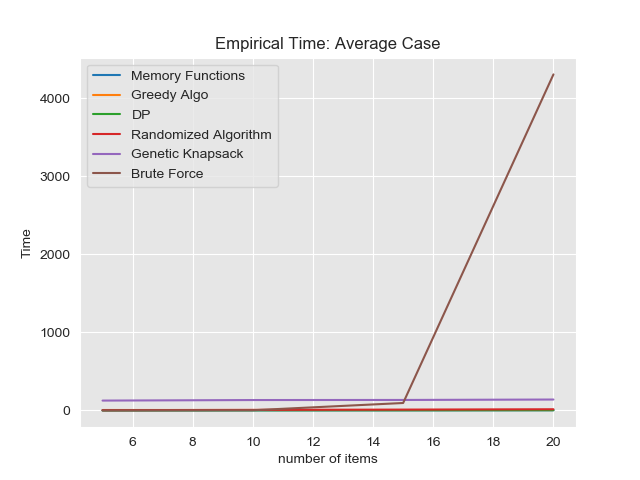
\includegraphics[scale=0.55]{BF/avgTime.png} \label{fig:avgTimeBF} 
  } 
  \subfigure[Without Brute force, for n=500]{% 
    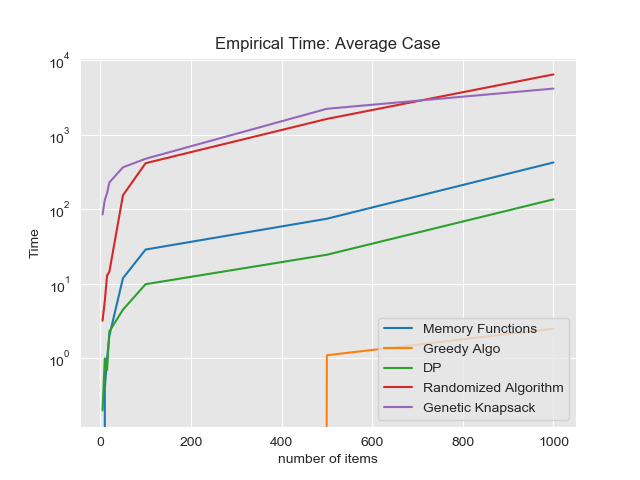
\includegraphics[scale=0.55]{avgTime.png} \label{fig:avgTime} 
  } 
  \caption{Average Time Analysis of Knapsack Problem} 
  \centering
  \label{fig:AvgTimeAnalysis}
\end{figure}

\autoref{fig:AvgTimeAnalysis} shows that our numerical solution matches our expectation. Brute force shoots off very soon (\autoref{fig:avgTimeBF}, and the randomized algorithm and genetic algorithm are the slowest, interestingly, memory functions and DP follow the same order, with memory function being the slower of the two, and greedy algorithm is the fastest. 


\begin{figure}[!ht] 
  \subfigure[With brute force, for upto n=20]{% 
    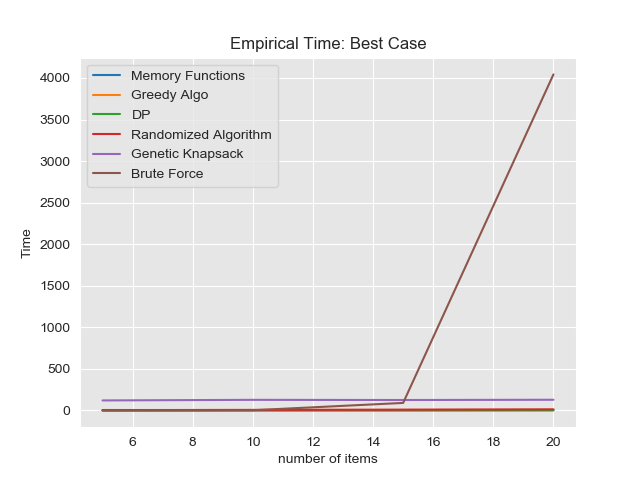
\includegraphics[scale=0.55]{BF/bestTime.png} \label{fig:BestTimeBF} 
  } 
  \subfigure[Without Brute force, for n=500]{% 
    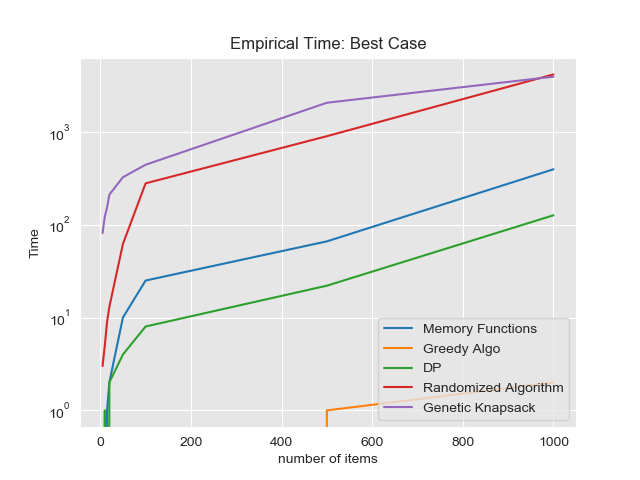
\includegraphics[scale=0.55]{bestTime.png} \label{fig:BestTime} 
  } 
  \caption{Best Time Analysis of Knapsack Problem} 
  \centering
  \label{fig:BestTimeAnalysis}
\end{figure}

The best case also follows our expectation in \autoref{fig:BestTime}, with greedy algorithm being the fastest, and randomized algorithm(s) performing the slowest. We can notice the best case time to be slightly less than average case, but the rate of growth is almost same.

\begin{figure}[!ht] 
  \subfigure[With brute force, for upto n=20]{% 
    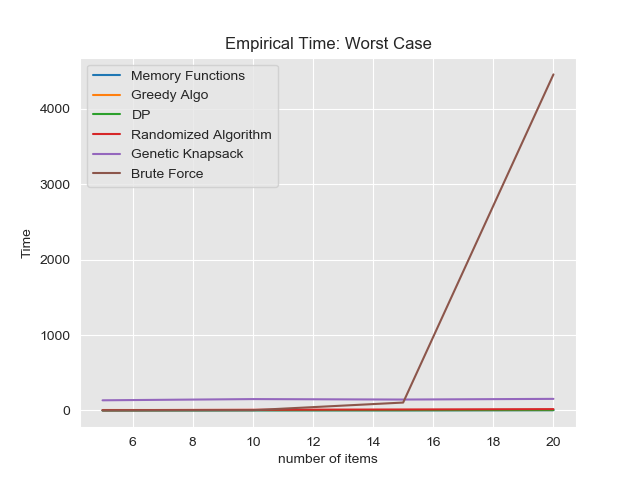
\includegraphics[scale=0.55]{BF/worstTime.png} \label{fig:WorstTimeBF} 
  } 
  \subfigure[Without Brute force, for n=500]{% 
    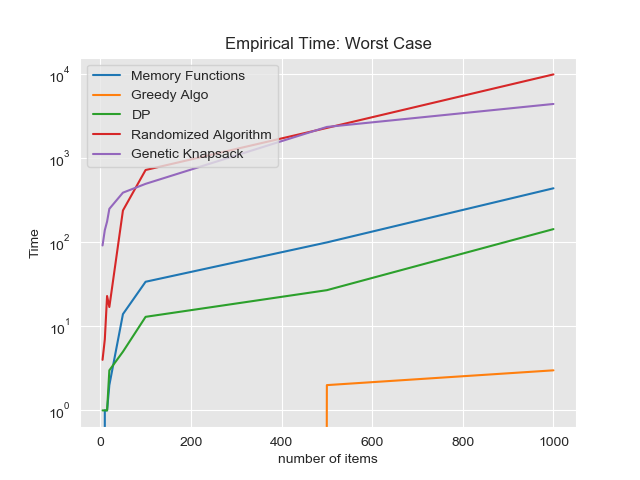
\includegraphics[scale=0.55]{worstTime.png} \label{fig:WorstTime} 
  } 
  \caption{Worst Time Analysis of Knapsack Problem} 
  \centering
  \label{fig:WorstMemoryAnalysis}
\end{figure}

In the worst case, genetic algorithm takes slightly less time than randomized, and their graphs overlap multiple times, other than that, the plot follows our general expectation.


\subsection{Space Analysis}
This refers to the analytical memory usage during the execution of the algorithm. We kept in account the size of memory allocated and calculated the number of memory accesses (either read or write) during the execution to arrays or (python lists) for each algorithm seperately to analytically analyze the memory accesses during the execution. 

Similar to the time analysis, we ran the algorithms 10 times each to average out the randomness, since the data is random.

\begin{figure}[!ht] 
  \subfigure[With brute force, for upto n=20]{% 
    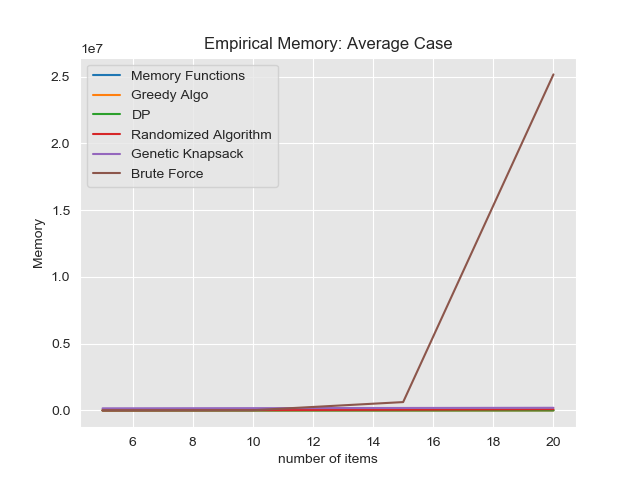
\includegraphics[scale=0.55]{BF/avgMem.png} \label{fig:avgMemBF} 
  } 
  \subfigure[Without Brute force, for n=500]{% 
    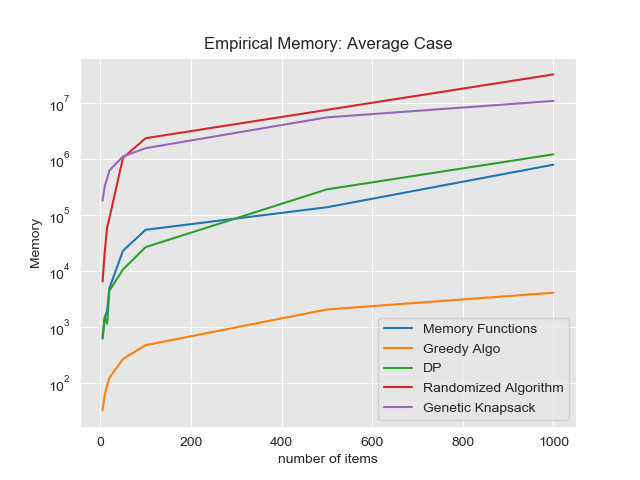
\includegraphics[scale=0.55]{avgMem.png} \label{fig:avgMem} 
  } 
  \caption{Average Memory Analysis of Knapsack Problem} 
  \centering
  \label{fig:AvgMemAnalysis}
\end{figure}

\begin{figure}[!ht] 
  \subfigure[With brute force, for upto n=20]{% 
    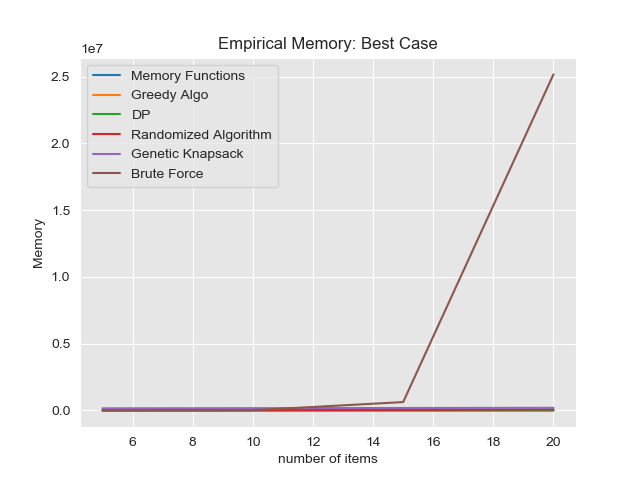
\includegraphics[scale=0.55]{BF/bestMem.png} \label{fig:BestMemBF} 
  } 
  \subfigure[Without Brute force, for n=500]{% 
    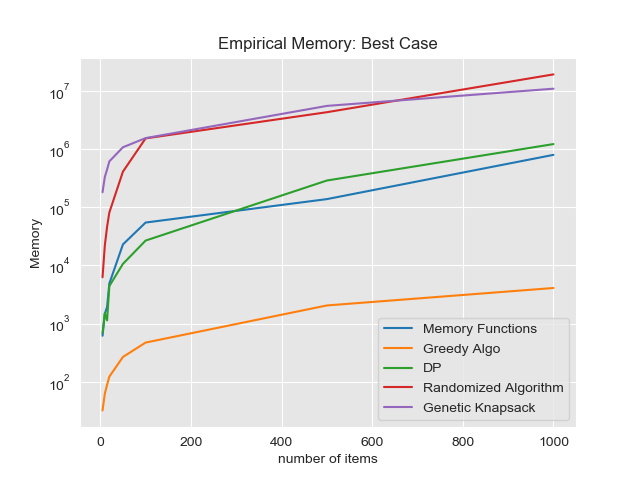
\includegraphics[scale=0.55]{bestMem.png} \label{fig:BestMem} 
  } 
  \caption{Best Memory Analysis of Knapsack Problem} 
  \centering
  \label{fig:WorstMemoryeAnalysis}
\end{figure}

\begin{figure}[!ht] 
  \subfigure[With brute force, for upto n=20]{% 
    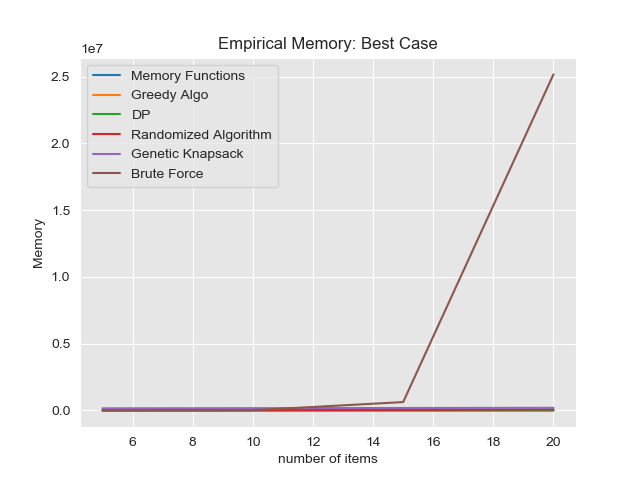
\includegraphics[scale=0.55]{BF/bestMem.png} \label{fig:WorstMemBF} 
  } 
  \subfigure[Without Brute force, for upto n=500]{% 
    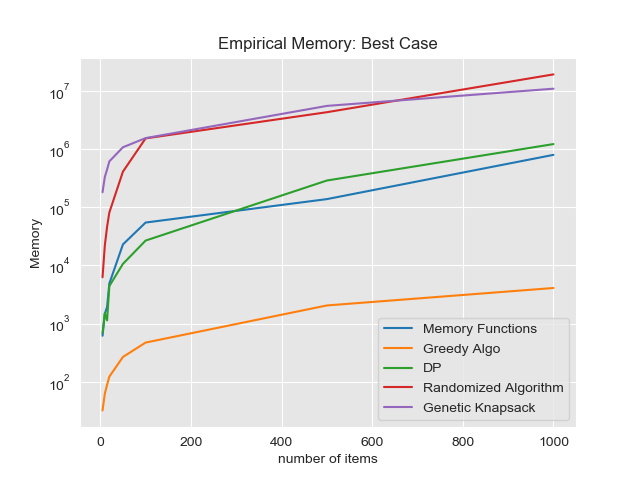
\includegraphics[scale=0.55]{bestMem.png} \label{fig:WorstMem} 
  } 
  \caption{Worst Memory Analysis of Knapsack Problem} 
  \centering
  \label{fig:WorstMemoryeAnalysis}
\end{figure}

\newpage

The results follow our expectation, we see how memory functions provide us an advantage over dynamic programming algorithms in terms of their accesses to memory. The memory functions have significantly less accesses to memory as they do not calculate the sub-problems which are not needed (unlike dynamic programming). Similarly, the randomized algorithms still have the highest amount of accesses to the memory and are the most costly.

\subsection{Correctness of Algorithm}
This refers to the distance of the output from each algorithm from the optimal solution. We obtained the optimal solution from dynamic programming algorithm, since it is always guaranteed to produce the optimal solution, and then we calculated the total weight of the solution, and used that weight as the benchmark to compare with the solutions obtained from the other algorithms. This helped in providing more context to the analysis of the algorithm, keeping in view its time and space complexity.

To compute this, we considered DP as the algorithm which produces optimal output, and computed its cost, and then we did the same for the outputs produced by different algorithms. We did this 10 times for every n, and computed the average to smooth out the randomness. 

We expected the following outcomes, 
\begin{enumerate}
    \item Memory Function and Brute Force to produce optimal solution
    \item Genetic Algorithm and Randomized Algorithm to produce solutions which are less than optimal solution
    \item Greedy Algorithm to also produce solutions close to optimal but not entirely optimal
\end{enumerate}



\begin{figure}[!ht] 
  \subfigure[With brute force, for upto n=20]{% 
    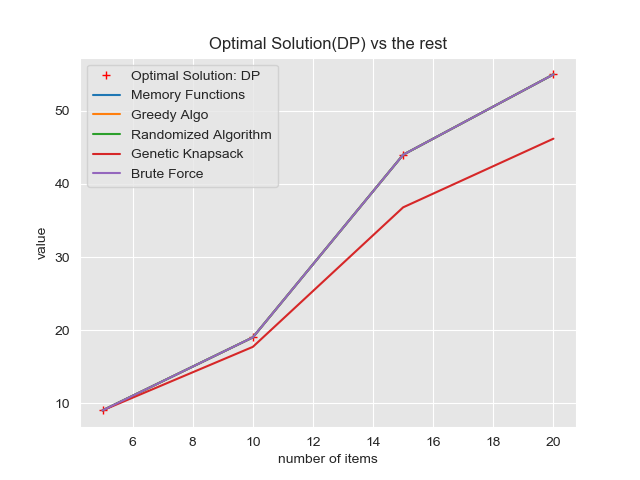
\includegraphics[scale=0.55]{BF/correctness.png} \label{fig:CorrectnessBF} 
  } 
  \subfigure[Without Brute force, for n=500]{% 
    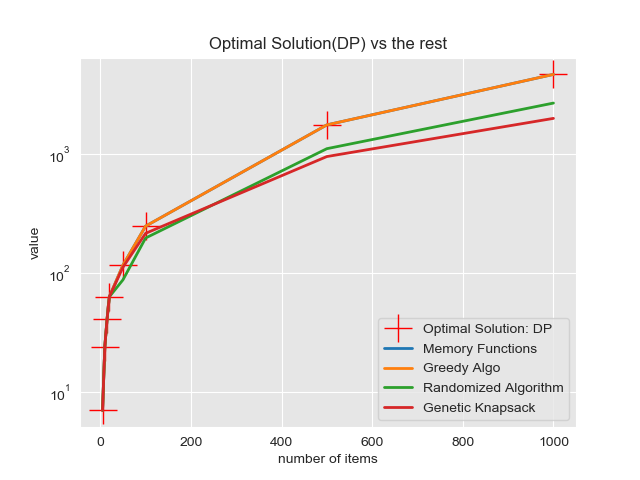
\includegraphics[scale=0.55]{correctness3.png} \label{fig:Correctness} 
  } 
  \caption{Correctness Analysis of Knapsack Problem} 
  \centering
  \label{fig:CorrectnessAnalysis}
\end{figure}

By looking at \autoref{fig:CorrectnessAnalysis}, we see that almost all of our expectations are met. We see that,

\begin{enumerate}
    \item We see that brute force algorithm (\autoref{fig:CorrectnessBF} and Memory functions (\autoref{fig:CorrectnessAnalysis}) always produce the most optimal solution.
    \item Randomized Algorithm and Genetic Algorithm produce solutions which are less than the optimal solution. Their lines overlap, which signify randomness and that we can not classify any of them as better than the other.
    \item Greedy algorithm provides the same (or almost the same) solution as the the optimal solution, which is slight contrary to our expectation. We realize this is probably because we tested the algorithm on a limited set of inputs, and that in a more general case, we can not expect greedy to produce the optimal solution. 
\end{enumerate}

% \newpage
% \section{Results}
% \begin{figure}[H] \begin{center}
%      
\includegraphics[width=0.8\columnwidth]{logo.png}
%         \caption{
%                 .caption here
%         } \end{center}
% \end{figure} 

\newpage 

\section{Conclusion}
In the comparative analysis of different approaches to solving the knapsack problem, we conclude that Dynamic Programming produces an \textit{optimal} solution in all cases regardless of the nature of the problem. Although genetic algorithm appears to take more time initially but with an increase in number of items the number of basic operations increase at approximately the same rate. However an increase in the capacity of the knapsack causes a greater space complexity in case of Dynamic programming. Thus, one may choose one approach over the other keeping in mind the space and time complexities according to the problem scenario. 
Brute Force continues to remain the slowest with a time complexity of $O(n2^n)$ and shoots off after the problem size of about 25 items. Memory functions is a recursive approach and works better than dynamic programming in terms of the number of computations but with an increase in the number of items, it takes a lot more memory and time to produce an output. Both Greedy and Randomized algorithm(Simulated annealing) do not guarantee an optimal solution with simulated annealing taking more time to converge to an optima.

\newpage
\begin{thebibliography}{99}


\bibitem{c1}
M. Hristakeva, D. Shrestha \href{http://www.micsymposium.org/mics_2005/papers/paper102.pdf}{``Different Approaches to Solve the 0/1 Knapsack Problem"} 

\bibitem{c2}
\href{https://github.com/TheAlgorithms/Python/blob/master/dynamic_programming/knapsack.py}{Memory Functions Solution to Knapsack 0/1 in Python} 
\bibitem{genetic}
\href{https://github.com/edmilsonrobson/0-1-Knapsack-Problem-with-Genetic-Algorithms}{Genetic Algorithm Solution to Knapsack 0/1 in Python} 

\bibitem{Dynamic Programming}
\href{https://rosettacode.org/wiki/Knapsack_problem/0-1#Python}{Dynamic Programming Solution to Knapsack 0/1 in Python}
\bibitem{Greedy Algorithm}
\href{https://www.sanfoundry.com/python-program-solve-fractional-knapsack-problem-using-greedy-algorithm/}{Greedy Algorithm Solution to Knapsack in Python}

\end{thebibliography}


\end{document}
